% generated by experiments/build_paper_assets.py -- do not edit by hand
\begin{figure}[t]
\centering
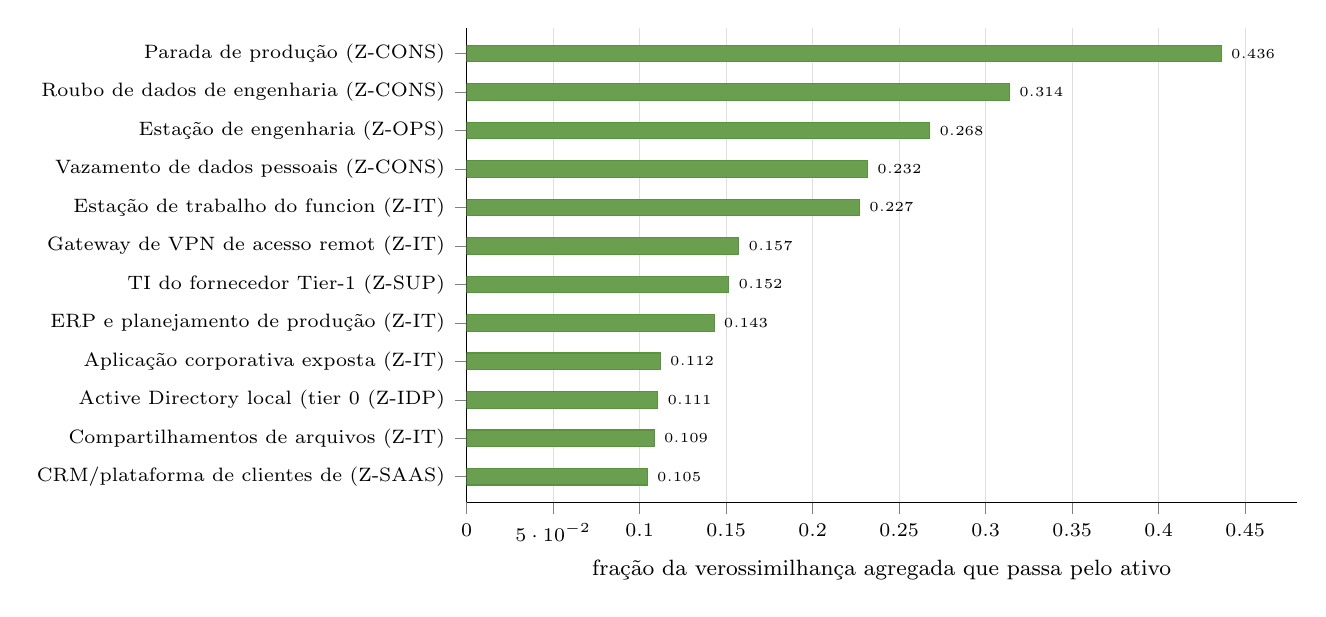
\begin{tikzpicture}
\begin{axis}[
    xbar, width=\linewidth, height=7.6cm,
    xlabel={fração da verossimilhança agregada que passa pelo ativo},
    xmin=0, enlarge y limits=0.06,
    ytick={0,1,2,3,4,5,6,7,8,9,10,11}, yticklabels={{Parada de produção (Z-CONS)},{Roubo de dados de engenharia (Z-CONS)},{Estação de engenharia (Z-OPS)},{Vazamento de dados pessoais (Z-CONS)},{Estação de trabalho do funcion (Z-IT)},{Gateway de VPN de acesso remot (Z-IT)},{TI do fornecedor Tier-1 (Z-SUP)},{ERP e planejamento de produção (Z-IT)},{Aplicação corporativa exposta  (Z-IT)},{Active Directory local (tier 0 (Z-IDP)},{Compartilhamentos de arquivos (Z-IT)},{CRM/plataforma de clientes de  (Z-SAAS)}},
    y dir=reverse, ticklabel style={font=\scriptsize},
    label style={font=\footnotesize},
    nodes near coords, nodes near coords style={font=\tiny},
    every node near coord/.append style={/pgf/number format/fixed,
        /pgf/number format/precision=3},
    xmajorgrids, grid style={gray!25}, axis lines*=left,
    bar width=6pt, tick align=outside,
]
\addplot[fill=OliveGreen!70, draw=OliveGreen!80] coordinates {
        (0.436200,0)
        (0.313800,1)
        (0.267700,2)
        (0.231800,3)
        (0.227200,4)
        (0.157400,5)
        (0.151600,6)
        (0.143100,7)
        (0.112000,8)
        (0.110500,9)
        (0.108500,10)
        (0.104500,11)
};
\end{axis}
\end{tikzpicture}
\caption{Pontos de estrangulamento da arquitetura de referência, ponderados por verossimilhança.}
\label{fig:chokepoints}
\end{figure}
